\documentclass[a4paper,oneside,12pt]{report}

%%%%%%%%%%%%%%%%%%% LOAD PACKAGES %%%%%%%%%%%%%%%%%%%%%
%Get support for äöüßÄÖÜ
\usepackage[utf8]{inputenc}
%Get support for word separation
\usepackage[T1]{fontenc}
%Direkte Verwendung von Umlauten
\usepackage[ansinew]{luainputenc}
%Get Support for US english and german
\usepackage[english,ngerman]{babel}
%verbesserter Randausgleich
\usepackage{microtype}
%zulässiger Wortzwischenraum erhöhen für noch besseren Randausgleich und Blocksatzbildung
\setlength\emergencystretch{1em}
%Einrücken nach Absatz für gesamtes Dokument abstellen
\setlength{\parindent}{0pt} 
%Bildbeschreibung zentrieren
\usepackage[center]{caption}
%Support for Graphics .png .jpg .pdf 
\usepackage{graphicx}
%Zusätzliche Option[H] bei Bildern - Hier und und sonst nirgends!
\usepackage{float}
%Adjust the page margins asymmetrical, Need to be before subfig
\usepackage[left=3cm, right=2.5cm, top=3cm, bottom=3cm, a4paper, portrait]{geometry}
%Kopf- und Fußzeilen
\usepackage{fancyhdr}
%für Fußnote (linksbündig)
\usepackage[flushmargin,bottom]{footmisc}
%Erweiterung des Mathematikmoduses
\usepackage{amsmath}
%Use Palatino Linotype 
\usepackage{mathpazo}
%Don´t show "Kapitel 1" at \chapter
\usepackage{titlesec} 
\titleformat{\chapter}{\bfseries\Huge}{\thechapter\quad}{0em}{}
%Abstand Kapitelüberschiften zum Kopfrand
\titlespacing{\chapter}{0pt}{*-2}{*1.5}
\usepackage{setspace}
\AtBeginDocument{\renewcommand{\chaptername}{}}
%Tabellenspalten/zeilen einfärben
\usepackage{colortbl}
%variable Tabellenbreite
\usepackage{tabularx}
%Multirow in Tabelle
\usepackage{multirow}
%Tabellenüberschrift links oben!
\usepackage[singlelinecheck=false]{caption}
%Programmcode einfügen
\usepackage{listings}
%Programmcode Farben ändern
\usepackage{xcolor}
%Hyperlink
\usepackage[colorlinks=true,linkcolor=black, citecolor=black, urlcolor=black]{hyperref}
%Ordnerstruktur erstellen
\usepackage{dirtree}
\usepackage{subfigure}
%Abkuerzungen
\usepackage{acronym}
%Highlighting
\usepackage{color,soul}
%Unterstützung für textumflossenes Bild 
\usepackage{wrapfig}
%Tabellen Linien
\usepackage{booktabs}


%//%%%%%%%%%%%%%%%%%% END LOAD PACKAGES %%%%%%%%%%%%%%%%%%%%
%//%%%%%%%%%%%%%%%%%% SETTINGS %%%%%%%%%%%%%%%%%%%%%%%%%
%Adjust headings and footers --> \usepackage{fancyhdr}
%Give the headings some space
\setlength{\headheight}{20pt}
%This is valid for all pages exept chapters
\pagestyle{fancy}

\fancyhf{} % clear all headers and footers
%Ausrichtung Kopf- /Fußzeile
\lhead[]{\fancyplain{}{\leftmark}}
\cfoot[]{\thepage}
\renewcommand{\headrulewidth}{0.4pt}
%For \chapters \maketitle
\fancypagestyle{plain}{%
	\fancyhf{} % clear all header and footer fields
	\cfoot[]{\thepage}%
	\renewcommand{\headrulewidth}{0pt}
	\renewcommand{\footrulewidth}{0pt}
}
%Deactivate command --> small letter
\let\MakeUppercase\relax
%Tiefe von Inhaltsverzeichnis 
\setcounter{secnumdepth}{3}
\setcounter{tocdepth}{3}
%Programmcodeeinstellungen
\lstset{
	backgroundcolor=\color{black!5},
	tabsize=4,
	language=C++,
	captionpos=b,
	tabsize=3,
	frame=lines,
	numbers=left,
	numberstyle=\scriptsize,
	numbersep=5pt,
	breaklines=true,
	showstringspaces=false,
	basicstyle=\scriptsize,
	%identifierstyle=\color{magenta},
	keywordstyle=\color[rgb]{0.8,0.4,0},
	commentstyle=\color[rgb]{0.9,0.3,0.9,},
	stringstyle=\color{green},
	emphstyle=\color{blue},
}
%Programmcodeeinstellungen, style Arduino
	\lstdefinestyle{Arduino}{%
		%style=numbers,
		keywords={soup},%                 define keywords
		%morestring=[s]{<}{>},%			  define <> as strings
		morecomment=[l]{\#},%             treat // as comments
		morecomment=[s]{/*}{*/},%         define /* ... */ comments
		emph={void, for, else, if, in, HIGH, OUTPUT, LOW, int, uint8_t, self, def, True, False, print, from, import, as, class, try, except, not, or, return, global},%        keywords to emphasize	
}


%Bennenung von Caption bei Programmcode 
	\renewcommand{\lstlistingname}{Programmcode}
	\renewcommand{\lstlistlistingname}{\lstlistingname}
	%Bennenung von Bilderquelle als "Quelle:"
	\newcommand*{\quelle}{%
		\footnotesize Quelle:
	}

%//%%%%%%%%%%%%%%%%%% END SETTINGS %%%%%%%%%%%%%%%%%%%%%%%%%

%\\%%%%%%%%%%%%%%%%%% DOCUMENT %%%%%%%%%%%%%%%%%%%%%%%%%


\begin{document}
	%%%%Bearbeitet
%Deckblatt
\thispagestyle{empty}
\begin{center}
	
\includegraphics[scale=0.5]{Bilder/HM1_logo.png}


	
	\vspace{1.5cm}
	\huge{Programmcode}\\\vspace{1.5cm}
	\large{im Zusammenhang mit der Bachelorarbeit}\\\vspace{0.5cm}
	\large{an der}\\\vspace{0.5cm}
	
	\huge{Hochschule München}\\
	\normalsize {für angewandte Wissenschaften}\\\vspace{0.5cm}
	\large{mit dem Titel}\\\vspace{1cm}
    \begin{center}
		\Huge{\textbf{Aufbau eines automatischen Testers für ein automotive Messtechnik Rack}}\\[2.0cm]
    \end{center}
    
	
	
	\large{Fakultät für Informatik und Mathematik}\\
	\normalsize {Studiengang Master Wirtschaftsinformatik}\\\vspace{2.1cm}
	
\end{center}

	
\newpage
\thispagestyle{empty}
\begin{flushleft}	
	\begin{tabular}[H]{ll}
		
		Ersteller: & \large{Johannes Knippel, Anja Wolf,}\\[0.2cm]
		 			& \large{Johanna Sickendiek, Skanny}\\[0,2cm]
		1. Prüfer:		  & \large{blablablabla}\\[0.2cm]
		2. Prüfer:		  & \large{loablebli}\\[.7cm]
		
		
		Betreuer an der Hochschule München: 	& \large{Prof. Dr. Rainer Schmidt}\\[0.5cm]
		Ausgabedatum:					& \large{19.03.2018}\\[0.5cm]
		Abgabedatum:					& \large{22.07.2018}\\[3.5cm]
	
		
		%FeldLinks für OrtDatum1	
		%\hspace*{\fill}
	
		\parbox{7cm}{\hrule\medskip Ort, Datum\\ [0.3cm]}	&	\parbox{7cm}{\hrule\medskip Unterschrift des 1. Prüfers\\ [0.2cm]Blaaaaaaaaaaaabla}\\[1.5cm]
		\parbox{7cm}{\hrule\medskip Ort, Datum\\ [0.31cm]}	&	\parbox{7cm}{\hrule\medskip Unterschrift des 2. Prüfers\\ [0.2cm]Blaaaaaaaaaaaabla}\\[1.5cm]
		\parbox{7cm}{\hrule\medskip Ort, Datum\\ [0.33cm]}	&	\parbox{7cm}{\hrule\medskip Unterschrift des Verfassers\\ [0.2cm]Johannes Knippel}\\[1.5cm]
		\parbox{7cm}{\hrule\medskip Ort, Datum\\ [0.33cm]}	&	\parbox{7cm}{\hrule\medskip Unterschrift des Verfassers\\ [0.2cm]Anja Wolf}\\[1.5cm]
		\parbox{7cm}{\hrule\medskip Ort, Datum\\ [0.33cm]}	&	\parbox{7cm}{\hrule\medskip Unterschrift des Verfassers\\ [0.2cm]Johanna Sickendiek}\\[1.5cm]
		\parbox{7cm}{\hrule\medskip Ort, Datum\\ [0.33cm]}	&	\parbox{7cm}{\hrule\medskip Unterschrift des Verfassers\\ [0.2cm]Skanny}\\
	\end{tabular}
\end{flushleft}

	
	
	

	\pagenumbering{Roman}


%												 Inhaltsverzeichnis
	\newpage
	\tableofcontents
	
	
	
	
	
%											    Kapitel 1 - Einleitung
	%\newpage
	\pagenumbering{arabic}
	\setstretch{1.5}
	\chapter[Problemstellung - Johannes Knippel]{Problemstellung}\label{probstellung}
	
		Für nahezu Jedermann bietet das WWW im Vergleich zu damaligen Zeiten ungeahnte Möglichkeiten der Recherche und Themenfindung. Noch nie waren so viele Informationen öffentlich einsehbar wie heute. Meist sind jedoch die gewünschten Inhalte an vielen unterschiedlichen Orten im Web verteilt, auf unterschiedlichste Weisen formatiert oder aufgrund schlechter Informationsarchitektur nur mit größerem Aufwand zu erreichen. Grundsätzlich kann die Fülle an Ergebnissen überfordern und nicht immer sind alle relevanten Inhalte über gängige Suchmaschinen auffindbar. Das bedeutet dann oft die mühsame Suche nach den relevanten Informationen in nicht immer nutzerfreundlich gestalteten Datenbanken. Bei so gut wie allen Recherchearbeiten besteht die Aufgabe heutzutage darin, die sprichwörtliche „Nadel im Heuhaufen“ zu finden. In vielen Fällen wünscht man sich einen gewissen Grad an Automatisierung. Daher soll im Rahmen eines Forschungsprojektes an der Hochschule München ein Tool entworfen werden, das Informationen und Inhalte von Webseiten automatisiert gewinnt. 
		\\
		Programmiertechnisch bedient man sich hierfür meistens vorhandener Schnittstellen, die die jeweiligen Quellen zur Verfügung stellen. Neben anwendungsspezifischen APIs sind dies zum Beispiel RSS- oder AtomFeeds, die in eigene Datenbanken geladen und von dort aus weiterverarbeitet werden können. \cite{bib-atomfeed} Die Informationen liegen in diesen Fällen also bereits in einem strukturierten Format vor und enthalten wenig bis gar keinen überflüssigen Inhalt.
		\\
		Hingegen wenn keine der genannten Schnittstellen angeboten werden, bleibt die ständige Beobachtung dieser Inhalte schwierig. Sofern es sich bei den Quellen um einfach strukturierte HTML-Seiten handelt, kann man sich mit verschiedenen Tools weiterhelfen. Gerade bei öffentlichen Datenbanken, deren Inhalte über Webformulare abgefragt werden („Deep Web“), ist dies jedoch meistens nicht möglich. \cite{bib-deepweb} Hier können Webscraper weiterhelfen, die das automatisierte „Auslesen“ von bestimmten strukturierten	oder semi-strukturierten Inhalten aus öffentlich zugänglichen Webseiten ermöglichen. 
		\\
		\newline
		Diese Studienarbeit beleuchtet am Beispiel von TripAdvisor wie ein solcher Webscraper implementiert werden kann. Des Weiteren umfasst diese Studienarbeit das automatisierte Abspeichern der gewonnenen Daten in einer strukturierten Datenbank.
		
		%Gewonnene Daten können so Aufschluss über Verhaltensweisen, Interessen und auch mögliche Kaufanregungen geben.
		

	\chapter{Grundlagen}\label{grlagen}
	
		Das folgende Kapitel geht auf grundlegende Datenstrukturen ein, beleuchtet das Thema Web Scraping, dessen Funktionsweise und Verwendung sowie die Beschreibung des Reiseinformationsportals TripAdvisor. 
	
		\section[Datenstrukturen - Johanna Sickendiek]{Datenstrukturen}
			
			Sowohl der Kontext von Daten, als auch ihre Eigenschaften führen zur Strukturierung dieser in verschiedene Datenarten. Kontextinformationen machen genauere Angaben zu Prozessen in denen die Daten benötigt werden. Eigenschaften hingegen unterscheiden Daten nach Format, Inhalt, Stabilität, Verarbeitung oder Struktur.
			\\
			Besonders relevant für dieses Projekt ist folglich letzteres – die Struktur von Daten. Hier unterscheidet man grundsätzlich zwischen drei verschiedenen Fällen, strukturierten, semistrukturierten und unstrukturierten Daten.
			\\
			Bei strukturierten Daten sind Metadaten, d.h. strukturgebende Informationen zu Daten vorhanden. Diese können u.a. Auskunft zu Format, erlaubten Werten oder semantischer Bedeutung geben. Ein klassisches Beispiel für strukturierte Daten sind alle möglichen Formen von Datenbanken. Hier müssen zunächst das Schema der Datenbank und deren einzelnen Tabellen festgelegt werden bevor Daten in die definierten Felder einfügt werden können. Somit ist eine einfache Analyse dieser zu einem späteren Zeitpunkt sichergestellt.
			\\
			Bei semistrukturierte Daten sind einzelne Bestandteile strukturiert, es mangelt jedoch an einer eindeutigen strukturierten Gesamtheit. Die Daten sind keinem objektorientierten oder relationalem Datenbankschema untergeordnet.
			\\
			Bei unstrukturierten Daten wird keinem eindeutigen Schema gefolgt, nur einer reinen Bitfolge. Das bedeutet jedoch nicht, dass die Daten gar keine Struktur aufweisen. Diese ist jedoch nicht direkt bzw. eindeutig für den Nutzer erkennbar. Neben Multimedia Daten (Bilder, Musik) finden sich unstrukturierten Daten auch meist in Emails, auf Internetseiten oder in Text-Dokumenten \cite{bib-daten}.
			\\
			Mithilfe von Web Scraping werden unstrukturierte Daten im Web zu Daten mit strukturgebenden Metadaten transformiert. Was genau Web Scraping bedeutet und wie es funktioniert, wird im nächsten Abschnitt näher erläutert.
			
			
		\section[Web Scraping - Johanna Sickendiek]{Web Scraping}
		
			Mit Web Scraping – auch “Web Harvesting”, “Web data mining” oder “Web data extraction“ genannt – wird das automatisierte herunterladen, analysieren und organisieren von Daten mehrerer Webseiten bezeichnet. Der Vorteil ist, dass aus einer Menge von unstrukturierten Informationen nur die benötigten Daten einer Webseite gezielt extrahiert und strukturiert abgespeichert werden. \cite{bib-webscraping}
			\\			
			Der Begriff „Scraping“ (engl.: „abkratzen, schaben“) gibt es circa so lange wie das Internet selbst. Bevor Web Scraping populär wurde war das Verfahren „Screen Scraping“ bereits allgemein bekannt. Damit wird das Auslesen von Daten aus Darstellungen am Computer bezeichnet. Genau wie heute war man damals schon daran interessiert, große Textmengen zu extrahieren, um daraus nur die benötigten Daten für den späteren Gebrauch zu speichern. Da dieses Verfahren heutzutage meist nur noch für Webseiten benötigt wird, wurde der Begriff „Web Scraping“ etabliert. \cite{bib-webscraping}
			\\
			Oft wird auch als Synonym der Begriff „Web Crawling“ verwendet. Beide Verfahren untersuchen Daten aus dem Internet, jedoch ist Web Crawling ein Prozess, der eine große Anzahl von Webseiten nach bestimmten Informationen durchsucht. Ein Beispiel dafür sind Suchmaschinen, wie beispielsweise Google, die mithilfe von Crawlern präzise Suchergebnisse anzeigen können. Im Gegenzug dazu ist Web Scraper ein Prozess, der nur bestimmte Informaionen einer begrenzten Auswahl von Webseiten sucht. Diese werden daraufhin in ein strukturiertes Format gebracht. \cite{bib-articlewebscraping}
			
			
			\subsection[Funktionsweise - Johanna Sickendiek]{Funktionsweise}
			
				Mithilfe von HTTP-Anfragen an eine ausgewählte URL wird der Inhalt einer Webseite – meist in Form von HTML – eingelesen. Dieser HTML-Code kann mithilfe von diversen Frameworks geparst werden, um die benötigten Daten zu erhalten. Die gängigste Technik, um diese Daten zu analysieren, ist mithilfe von HTML-Parsern. Sie konvertieren den HTML-Code in eine baumartige Struktur.  \cite{bib-scrapehero}
				\\
				Zur Extraktion der Daten ist es wichtig, dass sie eindeutig erkennbar sind. Die benötigten Informationen können beispielsweise mithilfe der Developer Tool-Ansicht einer Webseite untersucht werden und somit beispielsweise über einen eindeutigen Klassennamen oder einer ID identifiziert werden. Dabei sind die Daten auf vielen Webseiten nicht in dem benötigten Format und müssen zuerst bereinigt werden. Beispielsweise wird die durchschnittliche Anzahl an Sternen der Bewertungen eines Restaurants auf TripAdvisor (vgl. Abbildung \ref{pic-anzSterne}) als Bild dargestellt und nicht als Zeichenkette. \cite{bib-scrapehero}
				
				\begin{figure}[h]
					\centering
					\begin{minipage}[b]{0.9\textwidth}
						
\includegraphics[width=\textwidth]{Bilder/BeispielAnzahlSterne.png}
					\end{minipage}
					\centering
					\caption[Beispiel unbereinigte Daten]{Beispiel unbereinigte Daten} \cite{bib-anzSterne}
					\label{pic-anzSterne}
				\end{figure}
							
				Sobald alle Daten extrahiert und angepasst wurden, werden diese in einer dem Zweck angemessenen Form gespeichert. Diese Sicherung kann in Form von XML, JSON, CSV oder in einer Datenbank erfolgen. (vgl. Abbildung \ref{pic-webscraper2}) Somit ist eine weitere Verarbeitung der Daten möglich. \cite{bib-scrapehero}
				
				%TODO Wieso kommt das Bild hier nochmal vor? vgl Kap (Datenstrukturen)
				\begin{figure}[H]
					\centering
					\begin{minipage}[b]{0.6\textwidth}
						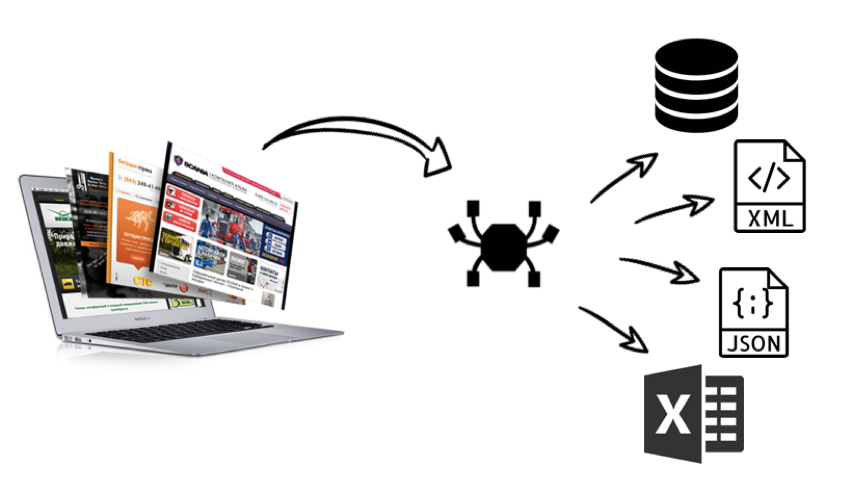
\includegraphics[width=\textwidth]{Bilder/Webcrawler.png}
					\end{minipage}
					\centering
					\caption[Funktionsweise eines Web Scrapers]{Funktionsweise eines Web Scrapers}
					\label{pic-webscraper2}
				\end{figure}
			
			
			\subsection[Verwendung - Johanna Sickendiek]{Verwendung}
			
				Aktuelle Softwares und Tools sind in der Lage, komplette Webseiten in strukturierte Daten umzuwandeln, um diese weiter zu verarbeiten. Dies kann in vielerlei Hinsicht nützlich sein. Denn alle Vorgänge, die manuell im Internet erfolgen, können somit automatisiert werden. Beispielsweise können Tickets für ein Konzert gekauft werden, sobald diese verfügbar sind, oder einen Onlineshop regelmäßig überprüfen, ob der Preis für einen bestimmten Artikel gesunken ist. \cite{bib-scrapehero}
				\\				
				In der folgenden Studienarbeit wurden die Informationen der Seite „TripAdvisor.de“ analysiert. Dieses Unternehmen wird im folgenden Kapitel näher betrachtet.
			
				
		\section[TripAdvisor - Johanna Sickendiek]{Tripadvisor}
	
			TripAdvisor ist eines der bekanntesten Bewertungsportale in der Touristik- und Hotelbranche.
			Auf dieser Webseite können User über 7,5 Millionen Restaurants, Unterkünfte, Airlines und Erlebnissen bewerten und vergleichen. Diese Bewertungen können sie zusätzlich mit Bildern veranschaulichen. Somit wird den Reisenden die Planung ihrer Reise vereinfacht, da sie mithilfe von echten Bewertungen einen authentischen Eindruck erhalten. 
			Zusätzlich bietet die Webseite im Bereich „Unterkünfte“ die Möglichkeit an, Zimmerpreise zu prüfen und diese direkt zu buchen. Mit insgesamt über 630 Millionen Bewertungen und Erfahrungsberichten der Reisenden und einem jährlichen Umsatz von mehr als 1,5 Milliarden Euro im Jahr 2017 \cite{bib-statista} ist TripAdvisor die weltweit größte Touristikwebseite. Sie ist auf 49 Märkten vertreten. \cite{bib-taMedia}
			
			\begin{figure}[H]
				\centering
				\begin{minipage}[b]{0.4\textwidth}
					
\includegraphics[width=\textwidth]{Bilder/LogoTripadvisor.png}
				\end{minipage}
				\centering
				\caption[TripAdvisor Logo]{TripAdvisor Logo} \cite{bib-tripadvisorLogo}
				\label{pic-taLogo}
			\end{figure}
			
			Jedoch ist diesen Bewertungsportalen nicht immer Glauben zu schenken. Mittlerweile gibt es Dienstleister, die für gute Bewertungen bezahlt werden. Denn TripAdvisor überprüft nur stichpunktartig, ob der Verfasser der Bewertung sich auch wirklich dort aufgehalten hat. \cite{bib-taSued}
	
	
	\chapter{Anforderungen}	
	
	    Der Anwender der Software soll in der Lage sein, sich ein auf dem Reiseportal „Tripadvisor“ (tripadvisor.com) verzeichnetes Restaurant auszusuchen und aus dieser Repräsentanz des Restaurants hinterlegte Informationen, insbesondere über Bewertungen von Usern des Portals, zu extrahieren. Diese Informationen sollen strukturiert auf einer beliebigen Datenbank persistiert und vom Anwender einsehbar sein.
	    \\
	    \\
       Im Folgenden werden die Anforderungen eingeteilt in funktionale und nicht–funktionale Anforderungen und werden näher erläutert.

       \begin{figure}[h]
				\centering
				\begin{minipage}[b]{1.0\textwidth}
					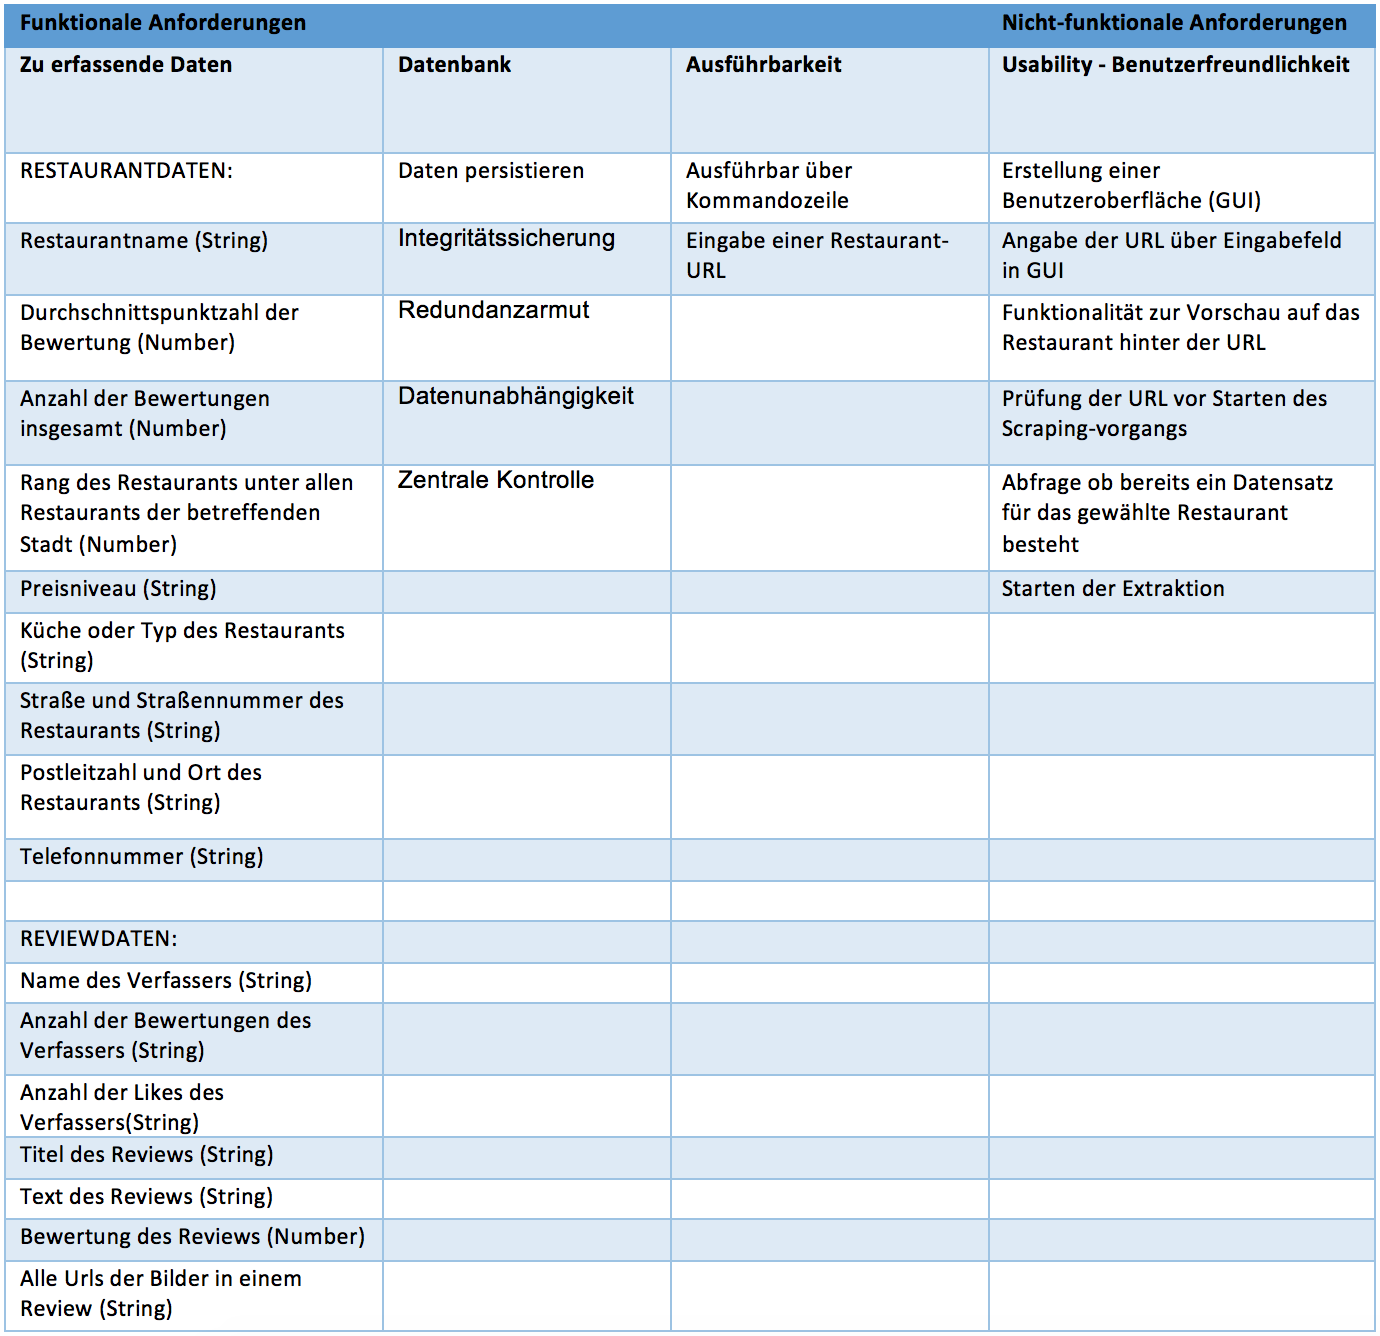
\includegraphics[width=\textwidth]{Bilder/TabAnforderungen.png}
				\end{minipage}
				\centering
				\caption[Anforderungsübersicht an das zu erstellende Programm]{Anforderungsübersicht an das zu erstellende Programm} 
				\label{TabAnforderungen}
			\end{figure}
	
		\section[Funktionale Anforderungen - Skanny Morandi]{Funktionale Anforderungen}

		\begin{description}
		\item[Zu erfassende Daten] Die zu extrahierenden Daten können in 2 Kategorien eingeteilt werden. Die 1. Kategorie besteht in Informationen zum konkreten Restaurant. So wie Name, Adresse, durchschnittliche Bewertungspunktzahl und weitere, wie aufgeführt in Tabelle \ref{TabAnforderungen}.  \\ 
        Die 2. Kategorie besteht aus den Bewertungen, die User auf dem Portal für dieses konkrete Restaurant abgegeben haben. Hier bestehen die Informationen von Interesse laut Anforderung aus dem Titel der Bewertung, dem Text der Bewertung, der abgegebenen Punktzahl sowie insbesondere der mit der Bewertung mitgesendeten Bilder. Von diesen wird laut Anforderung lediglich verlangt die auf die jeweiligen Bilder verweisenden URLs als Datenpunkt zu erfassen und nicht die Bildinformation selbst.

	
        \item[Datenbank Anforderungen]
        Nach der Extraktion von tripadvisor sollen die erfassten Daten persistiert werden um zu einem späteren Zeitpunkt für weitere Zwecke ohne großen Aufwand wieder verfügbar zu sein. Dies soll durch Eintragung in einer Datenbank realisiert werden. Weitere Anforderungen an diese Datenbank bestehen in: 
        \begin{itemize}
        \item Integritätssicherung – die Gewährleistung der Korrektheit der Datensätze auf der Datenbank durch entsprechende Prüfmaßnahmen bei Manipulation bzw. Eintragung von Datensätzen	    \\
        \item Redundanzarmut – Minimierung von doppelt geführten Datenpunkten oder -sätzen, sofern die Doppelung keine Mehrinformation beinhaltet \\
        \item Datenunabhängigkeit – das bearbeiten oder verwalten der in der Datenbank geführten Daten soll möglich sein ohne weitere Serverinfrastruktur o.ä. \\
        \item Zentrale Kontrolle – ein Administrator soll in der Lage sein, die gesamte Datenbank zu verwalten
        \\
        \end{itemize}
        \item[Ausführbarkeit des Anwenders] Der Empfänger bzw. Anwender der Software soll in der Lage sein die Programmfunktionalität zu starten und zu Beenden ohne weitere Abhängigkeiten. Als Voraussetzung wird hier angenommen, dass der Anwender über einen für den Stand der Zeit durchschnittlichen Rechner verfügt, auf dem es möglich ist ein Programm in der Kommandozeile des jeweiligen Betriebssystems auszuführen.
        \\
        \item[Eingabe einer Restaurant-URL] Der Anwender soll in der Lage sein dem Programm einen Parameter zu übergeben, der das Restaurant, dessen Daten extrahiert werden sollen, identifiziert. Im vorliegenden Kontext soll dies über die Eingabe der Tripadvisor-URL des betreffenden Restaurants erfolgen.
        \end{description}

	\section[Nicht funktionale Anforderungen - Skanny Morandi]{Nicht funktionale Anforderungen}
	
		Usability – Benutzerfreundlichkeit\\
        In Hinsicht darauf, dass die Anwender der Software nicht ausschließlich IT-affine Personen sein werden, soll die Ausführung der Software über eine einfach zu verstehende Graphische Benutzeroberfläche (GUI) erfolgen. 
        \\
        Die Eingabe der URL soll über ein Textfeld in der GUI gewährleistet werden. Bevor der Vorgang der Datenextraktion für das Restaurant und alle seine Bewertungen gestartet wird, soll es möglich sein über einen Button eine Validierung der angegebenen URL durchzuführen. Diese überprüft, ob die URL, zumindest Ihrer Form nach, eine gültige Tripadvisor-Restaurant-URL ist, und sicherstellen, dass das Programm nicht aus dem Grund fehlschlägt, dass die angegebene URL nicht die eines Tripadvisor-Restaurants ist.
        \\
        Anschließend an die Validierung sollen die Basisinformationen Name, PLZ und Ort sowie durchschnittliche Bewertung des mit der URL verbundenen Restaurants angezeigt werden. So kann sich der Anwender vor Starten des bis zu mehreren Minuten langen Vorgangs versichern, dass er auch wirklich die URL des gewünschten Restaurants angegeben hat.
        \\
        Letztendlich soll es möglich sein durch einen Button die Extraktion und Persistierung der Daten zu starten. Vor Starten des eigentlichen Vorgangs soll eine Prüfung erfolgen, ob das gewählte Restaurant bereits extrahiert wurde. Falls ja wird der Anwender entsprechend informiert und der Vorgang wird abgebrochen. 
	
	
	
	\chapter{Implementierung}\label{implementierung}
		
		Im folgenden Kapitel wird die voll umfängliche Implementierung des zu entwickelnden Web Scrapers beschrieben. Dabei wird zunächst auf die Konfiguration der Arbeitsumgebung eingegangen und die Hauptbibliothek von BeautifulSoup näher erläutert. Das Unterkapitel 'Implementierung WebCrawler' verdeutlicht anhand von Codebeispielen die Integration von Bibliotheken und die Extraktion der Rohdaten. Darauffolgend wird im Kapitel 'Datenhaltung' die Inklusion der Datenbank skizziert und im Abschluss die zum Programm entworfene Benutzeroberfläche erläutert.
	
		\section[Konfiguration - Anja Wolf]{Konfiguration}
		
			Zunächst wurde als Entwicklungsumgebung die aktuellste Version von Eclipse (Version 4.7.*) sowie als Programmiersprache die neueste Version von Python und PIP zur Verwaltung von Paketen installiert. Es wurde bewusst nicht die Version 2.7 verwendet, da ab der Version 3.0 Pakete, wie JSON und urllib, schon vorinstalliert sind. Es wurde Python gewählt, da dies die bekannteste Sprache für Web Scraper ist und Frameworks, wie Scrapy, Beautifulsoup, etc. in Python geschrieben sind. 
			\newline
			Um Python für Eclipse zu nutzen, wurde das Plugin „PyDev“ in Eclipse installiert. Daraufhin muss der Python-Interpreter konfiguriert werden. Diese Einstellung wird unter Window > Preferences vorgenommen. \cite{bib-pipEnv}
			\newline
			Für den Web Scraper wurden zunächst zwei wichtige Pakete mithilfe von PIP installiert: Requests und Beautifulsoup.
			Um die URL zu öffnen und den HTML Code der Webseite herunterzuladen, wird das Paket „Requests“ benötigt. Um diesen Code zu analysieren und die Daten zu extrahieren, wurde das Framework „Beautifulsoup“ installiert. \cite{bib-scrapeHero} 
			Warum sich in dieser Studienarbeit für dieses Framework entschieden wurde, wird im nächsten Abschnitt näher erläutert. 

	
		\section[BeautifulSoup - Anja Wolf]{BeautifulSoup}
		
			Für die Programmierung des Web Scrapers, um Daten von auf TripAdvisor gelisteten Hotels und Restaurants zu scrapen wurde die Python Library ‘BeautifulSoup‘ (\textit{bs4}) verwendet.
			\newline
			Hierbei handelt es sich um eine Library für XML und HTML parsing, die zunächst als zusätzliches Paket installiert werden muss. Beim Parsen werden XML oder HTML Dateien analysiert und auf ihre einzelnen Bestandteile geprüft. So können jegliche Informationen aus diesen Dateien gesucht bzw. extrahiert werden, vorausgesetzt es sind entsprechende Tags bzw. Attributnamen vorhanden. Ohne diese kann nicht gesucht werden \cite{bib-webpython}. Diese Einfachheit und gleichzeitig große Effizienz sind der westenliche Vorteil, warum das Projekt-Team sich für die Library BeautifulSoup und deren Methoden entschieden hat.
			\newline
			Um das wahrscheinlich am meisten verwendeten Objekt der BeautifulSoup Library – das BeautifulSoup Object – zu initialisieren, muss diesem ein XML bzw. HTML Dokument oder, wie in unserem Fall, der zu parsenden HTML-Code übergeben werden. BeautifulSoup kann eine URL also nicht selbstständig aufrufen, sondern erst mit dem gespeicherten Quelltext der HTML-Seite arbeiten \cite{bib-bs4}. In unserem Fall wird die TripAdvisor URL des gewünschten Hotels bzw. Restaurants daher zunächst mit einer Methode der Python Library \textit{‘request'} aufgerufen. Diese sendet einen HTTP/1.1 request und pingt die Website an, dass Informationen extrahiert werden möchten. Sobald der Webserver eine \textit{response} sendet wird der Inhalt der URL, d.h. der HTML-Code in einer einfachen String Variable gespeichert. Erst jetzt kann ein neues BeautifulSoup Object initialisiert werden (vgl. Programmcode 4.1).
			\begin{lstlisting} [caption={Initialisierung BeautifulSoup Object}\label{initbs4}, captionpos=b, style=Arduino]
			def get_single_data(self,url):
			source_code = requests.get(url)
			plain_text = source_code.text
			soup = BeautifulSoup(plain_text, "html.parser")
			\end{lstlisting}
			
			Dieses transformiert den komplexen HTML-Code in einen ebenfalls komplexen Baum mit Python Objekten. Die HTML-Tags korrespondieren mit den neuen Tag Objekten des BeautifulSoup Objects \cite{bib-bs4}. Am folgenden Beispiel kann die Struktur eines solchen beispielhaft veranschaulicht werden.
			
			\begin{figure}[H]
				\centering
				\begin{minipage}[b]{0.9\textwidth}
					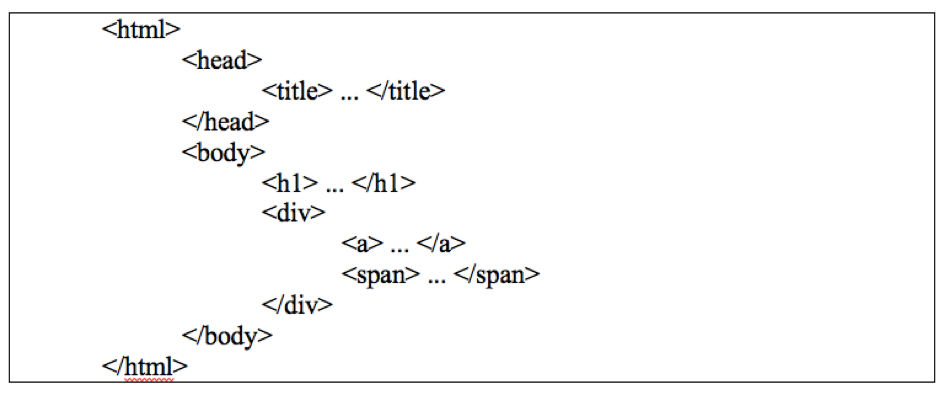
\includegraphics[width=\textwidth]{Bilder/HTMLcode.png}
				\end{minipage}
				\centering
				\caption[HTML Code bs4]{Baum mit Python Objekten \cite{bib-webpython}}
				\label{pic-HTMLcode}
			\end{figure}
			
			Natürlich enthält dieser normalerweise eine weitaus größere Anzahl an Vererbungen, d.h. ineinander verschachtelten Tags, und ist daher komplizierter zu lesen. Jedoch wird anhand dieses Beispiels bereits deutlich, wie die im folgenden beschriebenen Methoden der BeautifulSoup Library damit arbeiten können.
			\newline
			Sobald das BeautifulSoup Object vorliegt, können die vorhandenen Methoden der bs4 Library genutzt werden. In folgender Tabelle sind die beiden bekanntesten und auch im Programm-Code am meisten genutzten Methoden aufgelistet \cite{bib-bs4}.
		
			\begin{figure}[H]
				\centering
				\begin{minipage}[b]{0.9\textwidth}
					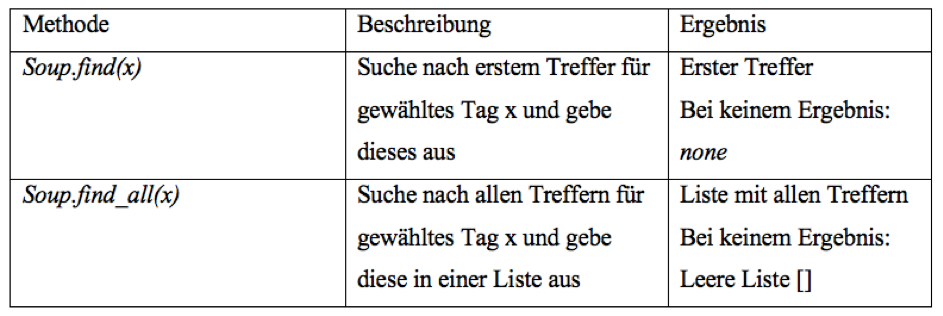
\includegraphics[width=\textwidth]{Bilder/SoupMethoden.png}
				\end{minipage}
				\centering
				\caption[Methoden bs4]{Such-Methoden der Python Library BeautifulSoup \cite{bib-bs4}}
				\label{pic-SoupMethoden}
			\end{figure}
			
			Im folgenden Kapitel werden diese genutzt um den Webcrawler für TripAdvisor erfolgreich zu implementieren.
	
	
		\section[Implementierung WebCrawler - Anja Wolf]{Implementierung WebCrawler}
			
			Im folgenden wird die Implementierung des Webcrawlers anhand von konkreten Code-Beispielen im Detail beschrieben. Besonders wird dabei auf die einfache und intuitive Verwendung der Bibliothek 'BeatifulSoup' eingegangen.
	
	
			\subsection[Initialisierung BeautifulSoup - Anja Wolf]{Initialisierung BeautifulSoup}
			
				Zunächst wird die URL des gewünschte Restaurants oder Hotels, für welches Daten extrahiert werden sollen, an die Methode \textit{get\_single\_data()} übergeben. Diese requested zu Beginn die übergebene URL, speichert ihren Source Code und initialisiert ein BeautifulSoup Object (vgl. Kapitel 4.2). Jetzt kann die eigentliche Implementierung des Webcrawlers beginnen. 
	
			\subsection[Extraktion Allgemeiner Daten - Anja Wolf]{Extraktion Allgemeiner Daten}			
				Zunächst sollen die in Kapitel 3 definierten allgemeinen Daten eines Restaurants bzw. Hotels extrahiert werden. Zu diesen gehören Name, Kontaktdetails, Küche, Preis-Level, Popularität, Anzahl an Bewertungen sowie die durchschnittlichen Bewertung. Dies soll in der neu definierten Methode \textit{get\_single\_data()}  mit den bereits beschriebene Suchfunktionen (Kapitel 4.2) umgesetzt werden.
				\\ 
				Die Unkompliziertheit von BeautifulSoup wird auch hier wieder deutlich. Mit \textit{find()} und \textit{find\_all()} kann nach jedem gewünschten Tag im Source Code gesucht und dessen Inhalt ausgegeben werden. So kann nach Strings, Blockelementen (z.B. <div>-Tag, Tabellen, Listen oder Überschriften), Inline-Elementen (z.B. <span>-Tag, Links oder Bilder) und weiteren Tags sowie deren Klassennamen gesucht werden \cite{bib-bs4}.
				Um diese zu bestimmen, ist es notwendig den übergebenen HTML-Code der URL genauer zu betrachten. Dies ist z.B. im Browser Chrome mit Rechtsklick „Quellcode anzeigen“ möglich. Um direkt auf ein gewünschtes Element im Quellcode zu springen, kann Rechtsklick „Element untersuchen“ genutzt werden. Diese Developer Tool-Ansicht ist deutlich strukturierter als den gesamten Text anzeigen zu lassen und erleichtert die Suche nach den gewünschten Tags um ein Vielfaches.
				\newline
				Der Programmcode 4.2 zeigt einige der Elemente und Klassen die gewählt wurden, um die gewünschten Informationen zu extrahieren.
				Um den Namen des Restaurants oder Hotels zu finden wird beispielsweise nach dem Tag \textit{<h1>} und dem class-Namen \textit{‘heading-title‘} gesucht. Dieser Tag steht üblicherweise für Überschriften und kommt meist nur einmal vor. Daher ist die Suche hier relativ simpel. Hingegen wird für die Durchschnittliche Bewertung des Restaurants oder Hotels nach einem \textit{<div>}-Tag mit class-Namen \textit{‘rs rating‘} gesucht. Da es sich dabei jedoch nur um die parent-class des gesuchten Tags handelt wird hier noch mit den Anhängen .div.span erweitert und tiefer in das BeautifulSoup Object „gezoomt“ um die children dieser Klasse zu erhalten. Mit der ID \textit{‘content‘} werden letztendlich die durchschnittliche Bewertung gefunden und in der Variable overallPoints gespeichert.
				\\
				\begin{lstlisting} [caption={Extraktion Allgemeiner Daten Object}\label{exallgdat}, captionpos=b, style=Arduino]
				for self.name in soup.find('h1', {'class': 'heading_title'}):
				print("Name:" + self.name.string)
				
				for self.rating_amount in soup.find('span', {'property': 'count'}):
				print("Anzahl Bewertungen:" + self.rating_amount.string)
				
				for self.cuisine in soup.find_all('span', {'class': 'header_links rating_and_popularity'}):
				print('Kueche:' + self.cuisine.text)
				\end{lstlisting}
				
				BeautifulSoup parsed so den gesamten HTML-Code nach den definierten Tag‘s und gibt je nach Methode das erste bzw. alle gefundenen Ergebnisse der Suche aus. Beispielsweise wird beim Namen nur nach einem Ergebnis gesucht, da hier mehrere Ergebnisse schlichtweg nicht sinnvoll wären. Bei der Art der Küche hingegen wird die Methode \textit{find\_all()} genutzt, da hier auch mehrere Ergebnissen gefunden werden können (vgl. Programmcode 4.2). Alle Ergebnisse werden wiederum in neu definierten Variablen als einfache Strings bzw. bei mehreren Ergebnissen in Listen gespeichert.
	
	
			\subsection[Bewertungslink aller Bewertungen auslesen - Anja Wolf]{Bewertungslink aller Bewertungen auslesen}
			
				Neben allgemeinen Daten zu Restaurant bzw. Hotel sollen außerdem noch Informationen zu allen Bewertungen inkl. angehängter Bilder und Daten zu deren Verfassern extrahiert und gespeichert werden. Dafür wird zunächst die URL jeder Bewertung generiert werden, um die Informationen von hier auszulesen. Da sich die Bewertungen meist nicht nur über eine, sondern eine Vielzahl an Seiten erstrecken wurde dies mit einer Verschachtelten for-Schleife gelöst.
				\newline
				Zunächst wurde eine for Schleife definiert, die alle verfügbaren Seiten eines Hotels oder Restaurants auf TripAdvisor durchläuft (vgl. Programmcode 4.3). Dafür wird die maximale Anzahl an Seiten mit \textit{find\_all()} gesucht und eine neue URL für jede der Seiten generiert. Diese unterschieden sich lediglich anhand eines Indexes (in 10er Schritten). Daher wird dieser für jeden Schleifendurchlauf, d.h. für jede Seite um 10 erhöht und mit der vorher gesplitteten URL neu zusammengesetzt. 
				\\
				\begin{lstlisting} [caption={For-Schleife über alle verfügbaren Bewertungsseiten}\label{forpages}, captionpos=b, style=Arduino]
				#create a new_url for each page of the reviews
				for index in range (10,pages*10, 10):
				
				data = url.split("Reviews-")
				new_url = data[0]+"Reviews-or"+str(index)+'-'+data[1]
				#pass the new_url to the loop_trough_review_pages function
				self.loop_through_review_pages(new_url)
				\end{lstlisting}
				
				Die neu generierte URL wird jedes Mal an die Methode \textit{loop\_through\_review\_pages()} übergeben.
				\\
				Mit dem ersten Aufruf von \textit{find\_all()} in dieser Mehtode wird zunächst nach dem \textit{<div>}-Tag mit class-Namen \textit{‘review container‘} gesucht (vgl. Programmcode 4.4). 
				\\
				\begin{lstlisting} [caption={Methode loop\_through\_review\_pages}\label{forcontainers}, captionpos=b, style=Arduino]
				def loop_through_review_pages(self, loop_url):
				source_code = requests.get(loop_url)
				plain_text = source_code.text
				soup = BeautifulSoup(plain_text, "html.parser")
				
				#get all review containers but on the nuw_url
				review_containers = soup.find_all('div', class_= 'review-container')
				reviewsPerPage = len(review_containers)
				
				#search trough all reviews on the page
				for container in review_containers:
				
				for link in container.find_all('a', href=True):
				href = "https://www.tripadvisor.de" + str(link.get('href'))
				#pass it to the function where single data is scraped
				self.get_single_review_data(href)
				\end{lstlisting}
				
				Bei einem solchen container handelt es sich um einen Block im HTML-Code, der alle Informationen einer einzigen Bewertung umfasst und diese sozusagen „einrahmt“. Für jede einzelne Bewertung wird dieser daher wiederholt (vgl. Abbildung \ref{pic-reviewcontainer}). Da die Methode \textit{find\_all()} genutzt wurde, wird deshalb in der Variable \textit{review\_containers} nun eine Liste mit allen ausgelesenen containern gespeichert.
				
				\begin{figure}[H]
					\centering
					\begin{minipage}[b]{0.9\textwidth}
						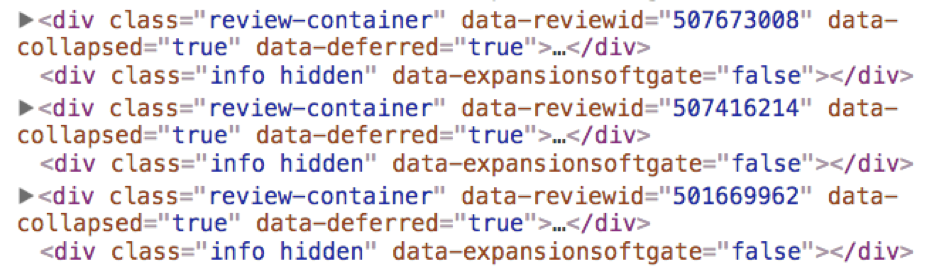
\includegraphics[width=\textwidth]{Bilder/reviewcontainer.png}
					\end{minipage}
					\centering
					\caption[Review Container]{Wiederholung der ‘review container' \cite{bib-reviewcontainer}}
					\label{pic-reviewcontainer}
				\end{figure}
			
				Mit dem erneuten Aufruf der Methode \textit{find\_all()} wird in einem container nach einem Link (\textit{<a>}-Tag) gesucht und gleichzeitig href auf \textit{‘True}‘ gesetzt. So stellt man sicher, dass nur Links mit href-Attribut ausgegeben werden. Bei diesem Link handelt es sich um den Teil der URL, der an die reguläre TripAdvisor Website angehängt werden muss, um die Bewertungsseite aufrufen zu können.
				\\
				Da jedoch nicht nur Informationen zur ersten gefunden Bewertung pro Seite, sondern zu allen Bewertungen extrahiert werden sollen, ist die Suchfunktion in eine weitere for-Schleife eingebunden. Diese loopt durch die vorher gespeicherte Liste \textit{review\_container}. So wird nicht nur der erste review container nach der Bewertungsseiten URL durchsucht sondern alle. Die Methode \textit{loop\_through\_review\_pages()} in Kombination mit der for-Schleife über alle Bewertungsseiten ermöglicht nun die Bewertungslinks jeder einzelnen Bewertung auszulesen.
				\newline
				Diese neu ausgelesene URL wird bei jedem Durchlauf an die Methode \textit{get\_single\_review\_data()} übergeben. Mit dieser können alle in Kapitel 3 definierten Daten zu den Bewertungen extrahiert werden.
	
	
	
			\subsection[Extraktion Bewertungensdaten - Anja Wolf]{Extraktion Bewertungensdaten}
			
				Die Daten der einzelnen Bewertungen werden mithilfe der oben genannten Methode 
				\textit{get\_single\_review\_data()} extrahiert. Dazu gehören wie in Kapitel 3 beschrieben: der Verfasser, seine Anzahl an Bewertungen und Likes, der Titel und der Text sowie die URL der Bilder einer Bewertung, falls dieser welche hochgeladen hat. 
				Zunächst wird wieder ein BeautifulSoup Object initalisiert, jedoch diesmal mit dem gespeicherten HTML-Code einer einzelnen Bewertungsseite (vgl. Programmcode 4.5).
				\\
				\begin{lstlisting} [caption={Initialisierung BeautifulSoup Object}\label{forpages}, captionpos=b, style=Arduino]
				def get_single_review_data(self,review_url):     
				source_code2 = requests.get(review_url)
				plain_text2 = source_code2.text
				soup = BeautifulSoup(plain_text2, "html.parser")
				\end{lstlisting}
				
				Die allgemeine Schwierigkeit an der Extraktion der Bewertungsdaten lag daran, dass auf der Webseite jeder einzelnen Bewertung zusätzlich noch die folgenden vier Bewertungen angezeigt werden. Dadurch, dass jede Bewertung den gleichen Aufbau an Klassen besitzt, war es nicht möglich nur nach dem Klassennamen zu suchen, da sonst beispielsweise die Überschriften aller Bewertungen ausgegeben worden wären. 
				Da der Name des Verfassers der Bewertung an erster Stelle im Quellcode angezeigt wird, kann dieses Element lediglich mithilfe der Methode 	\textit{find()} und dem Klassennamen ausgegeben werden. 
				Die Elemente „Anzahl an Bewertungen“ sowie „Anzahl an Likes“ besitzen jedoch denselben Klassennamen. Daher wurde in diesem Fall die Methode \textit{findAll()} benutzt, allerdings mit der Kombination, dass nur ein bestimmtes Element ausgegeben werden soll (vgl. Programmcode 4.6)
				\newpage
				\begin{lstlisting} [caption={Anzahl an Bewertungen und Likes des Verfassers}\label{forpages}, captionpos=b, style=Arduino]
				for self.numberOfReviews in soup.findAll('span', {'class': 'badgetext'})[0]:
				print("Anzahl Reviews: " + self.numberOfReviews.string)
				
				for self.numberOfLikes in soup.findAll('span', {'class': 'badgetext'})[1]:
				print("Anzahl Likes: " + self.numberOfLikes.string)
				\end{lstlisting}
				
				Somit wird für die Anzahl an Bewertungen der Text des ersten gefundenen Klassennamens ausgegeben, für die Anzahl an Likes der Text des zweiten Klassennamens. 
				Um den Titel sowie den Text der Bewertung zu extrahieren, wurde das JSON des heruntergeladenen HTML-Codes wieder in ein JSON-Format geparst (vgl. Programmcode 4.7). Denn die Problematik hierbei war, dass wenn die Bewertung in einer anderen Sprache verfasst worden ist, die Überschrift und der Text der Bewertung automatisch ins Deutsche übersetzt worden sind. Dadurch erkennt das System die übersetzte Überschrift sowie den Text anhand des Klassennamens nicht. Mithilfe dieses JSONs wurde zusätzlich die Anzahl an vergebenen Punkten herausgelesen.  
				\\
				\begin{lstlisting} [caption={Transformation in ein JSON-Format}\label{forpages}, captionpos=b, style=Arduino]
				self.item_name = soup.find('script', {'type': 'application/ld+json'})
				json_string = str(self.item_name.string)
				obj = json.loads(json_string)
				\end{lstlisting}
				
				
				Des Weiteren war die Anforderung, die URL der Bilder einer Bewertung abzuspeichern. Hierbei war die Schwierigkeit, dass auch Bewertungen ohne Bilder existieren. Des Weiteren können auch die anderen angezeigten Bewertungen auf der Webseite Bilder enthalten. Dadurch war es nicht möglich nur nach der Klasse \textit{inlinePhotosWrapper} zu suchen. Somit hätte das System auch die URLs der anderen Bewertungsbilder ausgegeben.  
				Daher sucht der Web Scraper zunächst, nach einer ID, die nur die gewünschte Bewertung besitzt. Daraufhin überprüft das System, ob es innerhalb dieser ID eine Klasse \textit{inlinePhotosWrapper} existiert, also ob der Verfasser der Bewertung Bilder hochgeladen hat. Ist dies der Fall, werden die URLs der Bilder in der Datenbank abgespeichert. Andernfalls wird eine textuelle Nachricht ausgegeben, dass für diese Bewertung keine Bilder hochgeladen wurden.
				\\
				\begin{lstlisting} [caption={Extraktion der URL der Bewertungsbilder}\label{forpages}, captionpos=b, style=Arduino]
				for link in soup.findAll('div', {'id': 'taplc_location_reviews_list_sur_callout_0'}):
				if link.find('div', {'class': 'inlinePhotosWrapper'}):
				for pic in link.findAll('img', {'class': 'centeredImg'}):
				self.src = pic.get('src')
				print("Quelle Bild " + self.src)
				else:
				print("No pictures have been uploaded for this review!")
				\end{lstlisting}
				
				Alle Ergebnisse werden wiederum in neu definierten Variablen als einfache Strings bzw. bei mehreren Ergebnissen in Listen gespeichert. 
			
		\section[Datenhaltung - Johannes Knippel]{Datenhaltung}\label{datenhaltung}
		%Einfach suche der Daten
			Eine Anforderung an das System besteht auch darin die gewonnenen Daten in einer Datenbank ablegen zu können. Zunächst wurden vom Product Owner die nötigen Ansprüche an die Datenbank bereitgestellt, nach der sich dann aus zwei Datenbanktypen eine vorteilhaftere herauskristallisieren konnte. 
			\\
			Da die gewonnen Rohdaten sich noch meist in einem encodierten Zustand befinden, müssen diese zunächst einen Bereinigungsprozess durchlaufen bevor sie leserlich in der Datenbank abgelegt werden können. Nicht nur das einfache Lesen der Daten sondern auch die Suche nach bestimmten Rechercheergebnissen soll möglichst intuitiv für den Nutzer ablaufen. Die Datenbankstruktur wurde daher Zusammen mit dem Auftraggeber abgestimmt und daraufhin die Architektur implementiert.
		
			\subsection[Definition der Datenbankanforderungen - Johannes Knippel]{Definition der Datenbankanforderungen}
			
				Die vom Abnehmer vordefinierten Anforderungen an die Datenbank sind wie folgt:
				%Stichpunkte DB-Anforderungen															
				\begin{itemize}
					\item Integritätssicherung\\
					\begin{small}
						Daten werden auf Korrektheit (bereits während der Eingabe) überprüft und Fehlmanipulationen  verhindert 
					\end{small}
					
					\item Redundanzarmut\\
					\begin{small}
						es gibt keine ungeordnete Mehrfachspeicherung von Datenwerten
					\end{small}
								
					\item Datenunabhängigkeit\\
					\begin{small}
						die Datenbank kann ohne Server verwaltet und weiterentwickelt werden
					\end{small} 
					
					\item zentrale Kontrolle\\
					\begin{small}
						ein Administrator ist in der Lage, das gesamte System von einem Rechner aus zu verwalten
					\end{small}
				\end{itemize}
				
				
				\subsubsection[Vergleich: SQLLite und TinyDB - Johannes Knippel]{Vergleich: SQLLite und TinyDB}
				
					Im Folgenden werden zwei NoSQOL Datenbanktypen miteinander verglichen, die dem Entwicklerteam als am sinnvollsten erschienen.
					\\
					\newline
					\underline{\textbf{TinyDB:}}
					\newline TinyDB ist eine leichtgewichtige dokumentenorientierte Datenbank, die für eine einfache Bedienung optimiert ist. Dabei ist sie in reinem Python geschrieben und hat keine externen Abhängigkeiten. Das Ziel sind kleine Apps, die von einer SQL-DB oder einem externen Datenbankserver entkoppelt funktionieren. \cite{bib-tinydb}
					\\
					\newline					
					\underline{\textbf{SQLite:}}
					\newline SQLite ist eine gemeinfreie Programmbibliothek, die ein relationales Datenbanksystem enthält. Sie unterstützt einen Großteil der im SQL-92-Standard festgelegten SQL-Sprachbefehle. Die SQLite-Bibliothek lässt sich direkt in entsprechende Anwendungen integrieren, sodass keine weitere Server-Software benötigt wird. Dies ist der entscheidende Unterschied zu anderen Datenbanksystemen. Durch das Einbinden der Bibliothek wird die Anwendung um Datenbankfunktionen erweitert, ohne auf externe Softwarepakete angewiesen zu sein. \cite{bib-sqlite}
					\\
					\newline Der wesentliche Vorteil von TinyDB liegt darin, dass diese Datenbank bereits in Python geschrieben ist und sich somit ideal in unseren Source-Code integrieren lässt. Es entstehen dabei keine Inkonsistenzen oder fehlerhafte Bibliotheksaufrufe. Ein weiteres Plus ist die Möglichkeit das Dateiformat JSON als Datenbank zu verwenden. Dieses kann im Vergleich zur SQLite Datei in sehr vielen Anwendungen integriert werden. Fortwährend ist man zu der Entscheidung gekommen, dass das Programmieren in SQL-Sprache in einem Python-Code zu Verwirrungen und unnötigen Programmier-Anforderungen beiträgt, was bei SQLite der Fall ist.
					\\
					Für das Projekt wurde sich einstimmig für die Verwendung von TinyDB als Datenbanksystem entschieden.
					
							
			\subsection[Datenbankstruktur - Johannes Knippel]{Datenbankstruktur}
			
				%Wie viele Tabellen, IDs, Verknüpfungen, Primärschlüssel
				Die extrahierten Daten können in grob vier Cluster eingeteilt werden, dabei bildet der erste Cluster die allgemeinen Daten des Restaurants, wie dessen Namen und Adresse. Den zweiten und dritten Cluster kann zusammenfassend als Benutzerdatenbank und Bewertungstext sehen. Der vierte Cluster bildet die Tabelle in der die Bilder abgespeichert werden, die zu einem jeweiligen Kommentar hinterlegt wurden.
				
				\subsubsection[Tabellen mit Spalten - Johannes Knippel]{Tabellen mit Spalten}\label{db_structure}
				
					Für die bessere Übersicht wurden in der Datenbank vier Tabellen angelegt, die wie folgt in ihre jeweiligen Spalten zerlegt sind:
					
					Cluster eins, Restaurant-Daten:
					
					\begin{table}[htbp]
						\centering
						\begin{tabular}{ccccc}
							\toprule
							\tiny \bf R\_ID & \tiny \bf RESTAURANTNAME & \tiny \bf PUNKTESKALA & \tiny \bf ANZAHL\_BEWERTUNGEN & \tiny \bf POPULARITAET\\
							\midrule
							\tiny atoincrement ID des Restaurants & \tiny Name des Restaurants & \tiny Gesamtbewertung & \tiny Anzahl abgegebener Bewertungen & \tiny Beliebtheitsgrad\\
							\bottomrule
						\end{tabular}
						\caption[Restaurant Tabelle Teil 1]{Tabelle der Restaurant-Daten Teil 1}
						\label{tab_rest1}
					\end{table}
				
					Fortsetzung:
					
					\begin{table}[htbp]
						\centering
						\begin{tabular}{ccccc}
							\toprule
							\tiny \bf PREIS\_LEVEL & \tiny \bf KUECHE & \tiny \bf STRASSE & \tiny \bf PLZ\_ORT & \tiny \bf TELEFONNUMMER\\
							\midrule
							\tiny Preislevel zw. 1 und 4 & \tiny Küchennationalität & \tiny Straßenname & \tiny Postleitzahl und Ort & \tiny Festnetznummer\\
							\bottomrule
						\end{tabular}
						\caption[Restaurant Tabelle Teil2]{Tabelle der Restaurant-Daten Teil 2}
						\label{tab_rest2}
					\end{table}
				

					Der zweite Cluster enthält sämtliche Daten von Benutzern, die eine Bewertung zum Restaurant abgegeben haben. Dieser teilt sich in folgende Tabellenstruktur auf:
				 	
				 	\begin{table}[htbp]
				 		\centering
				 		\begin{tabular}{cccc}
				 			\toprule
				 			\tiny \bf U\_ID & \tiny \bf REV\_ID & \tiny \bf BENUTZERNAME & \tiny \bf ANZAHL\_REVIEWS \\
				 			\midrule
				 			\tiny autoincrement ID des Users & \tiny autoincrement ID des Bewertungstextes & \tiny Benutzername & \tiny Anzahl der abgegebenen Bewertungen \\
				 			\bottomrule
				 		\end{tabular}
				 		\caption[Benutzer Tabelle]{Tabelle der Benutzer-Daten}
				 		\label{tab_user}
				 	\end{table}
			 	
			 		Cluster drei enthält den Bewertungstext und die dazugehörigen Attribute wie Titel und Rating:
			 		
			 		\begin{table}[H]
			 			\centering
			 			\begin{tabular}{cccccc}
			 				\toprule
			 				\tiny \bf R\_ID & \tiny \bf U\_ID & \tiny \bf REV\_ID & \tiny \bf TITEL & \tiny \bf BEWERTUNG & \tiny \bf RATING\\
			 				\midrule
			 				\tiny autoincrement ID des Restaurants & \tiny autoincrement ID des Benutzers & \tiny autoincrement ID der Bewertung & \tiny Titel & \tiny Bewertungstext & \tiny Rating des Textes\\
			 				\bottomrule
			 			\end{tabular}
			 			\caption[Bewertungs Tabelle]{Tabelle der Bewertungs-Daten}
			 			\label{tab_rev}
			 		\end{table}
				 	
				 	Der vierte Cluster enthält die direkten Links zu den hinterlegten Kommentar-Bildern:
				 	
				 	\begin{table}[H]
				 		\centering
				 		\begin{tabular}{cc}
				 			\toprule
				 			\tiny \bf REV\_ID & \tiny \bf QUELLE\\
				 			\midrule
				 			\tiny autoincrement ID der Bewertung & \tiny Link des Bildes\\
				 			\bottomrule
				 		\end{tabular}
				 		\caption[Bilder Tabelle]{Tabelle der Kommentar-Bilder}
				 		\label{tab_pics}
				 	\end{table}
			 	
			 	
				\subsubsection[Zeichnung und Zusammenhang - Johannes Knippel]{Zeichnung und Zusammenhang}
				
					Die Datenbank kann im angelegten Schema, wie es in Kapitel \ref{db_structure} beschrieben ist, über die autoincrement ID's der jeweiligen Tabellen durchsucht und verknüpft werden. Beim Anlegen der autoincrement ID's wurde darauf geachtet, dass keine ID mehrfach vorkommt. So kann dem Anwender eine verwechslungsfreie Suche garantiert werden.\\
					Ein Bewertungstext, der zu einem bestimmten Restaurant abgegeben wurde, kann beispielsweise mit folgendem Python-Code aufgerufen werden:
					\\
					\begin{lstlisting} [caption={Datenbanksuche: Reviews passend zum Restaurant}\label{dab_search}, captionpos=b, style=Arduino]
					result = db.search((where('RESTAURANTS')['R_ID']) == (where('REVIEWS')['R_ID']))
					print(result)
					\end{lstlisting}
					


			\subsection[Daten bereinigen und integrieren - Johannes Knippel]{Daten bereinigen und integrieren}
				
				Meist sind die Daten auf den Webseiten bereits kodiert im UTF-8 Muster hinterlegt. UTF-8 (Abk. für 8-Bit UCS Transformation Format, wobei UCS wiederum Universal Character Set abkürzt) ist die am weitesten verbreitete Kodierung für Unicode-Zeichen. Es ist in den ersten 128 Zeichen (Indizes 0–127) deckungsgleich mit ASCII und eignet sich, mit in der Regel nur einem Byte Speicherbedarf, für Zeichen vieler westlicher Sprachen besonders für die Kodierung englischsprachiger Texte. \cite{bib-utf8} Die bei TripAdvisor angewendete Kodierung ist in dem Fall auch UTF-8 und muss neu decodiert werden, um die deutschen Umlaute korrekt anzeigen zu können.
				\\
				Nachdem die Rohdaten in Variablen abgelegt wurden, können diese in einer neuen Methode für den Reinigungsprozess weiterverwendet werden. Zunächst wird eine Datenbankabfrage gestartet, bei der überprüft wird, ob der neu-gefundene Eintrag bereits in der Datenbank existiert. Ist dies der Fall wird ein Pop-Up-Fenster geöffnet, das beispielsweise bei der Restaurantabfrage einen Beenden-Button enthält, sodass nicht alle Daten zum Restaurant erneut eingefügt werden. Wird ein doppelter Eintrag hingegen bei einer Bewertung gefunden, kann das Pop-Up-Fenster einfach weg geklickt werden und das Programm läuft weiter. (vgl. Programmcode 4.7, Zeilen 3-12)
				\\
				Ist kein Eintrag vorhanden, werden die Daten zunächst in einem Array gespeichert und dann in der Datenbank abgelegt. Zuvor findet noch eine Decodierung der Rohdaten statt (vgl. Programmcode 4.7, Zeile 15).
				\\			
				\begin{lstlisting} [caption={Rohdaten decodieren und in Datenbank integrieren}\label{integration}, captionpos=b, style=Arduino]
				#HANDLE RESTAURANTS
				#check if there already exists an entry in the Restaurans-table with the same name and the same address (these two attributes don't change/are not variable so there is a more constant way to check for duplicates)
				if tableRestaurants.contains((where('RESTAURANTNAME') == self.name.string) & (where('PLZ_ORT') == self.locality.string)): 
					#pop up a message box
					msg = "Dieses Hotel hast du bereits gesucht und ist in der Datenbank hinterlegt!"
					popup = tk.Tk()
					popup.wm_title("!")
					label = ttk.Label(popup, text=msg)
					label.pack(side="top", fill="x", pady=10)
					B1 = ttk.Button(popup, text="Okay und Beenden", command = self.endProgram)
					B1.pack()
					popup.mainloop()
				# if there is no such entry, parse the data into the corresponding table of the database and define the data to insert into database including an auto increment ID for each Table       
				else:
					self.popularity2 = unicodedata.normalize('NFD', self.pupularity.text)
					print("Preis_Level: " + self.price_level)
					dataRestaurants = {'R_ID':self.idRestaurant, 'RESTAURANTNAME':self.name.string, 'PUNKTESKALA':self.overallPoints.div.span['content'], 'ANZAHL_BEWERTUNGEN':self.rating_amount.string, 'POPULARITAET':self.popularity2, 'PREIS_LEVEL':self.price_level, 'KUECHE':self.cuisine.text, 'STRASSE':self.address.string, 'PLZ_ORT':self.locality.string, 'TELEFONNUMMER':self.phonenumber.text}
					tableRestaurants.insert(dataRestaurants)
				\end{lstlisting}
				
				
		\section[Graphische Benutzeroberfläche - GUI - Skanny Morandi]{Graphische Benutzeroberfläche - GUI}\label{GUI}
		    Um der nicht-funktionalen Anforderung einer gewissen Usability über eine Graphische Benutzeroberfläche (GUI) nachzukommen wurde die Library „Tkinter“ genutzt. Tkinter ist ein integraler Bestandteil von Python3, ist „robust, schnell und plattformunabhänigig lauffähig“ \cite{bib-tkinterDocu}. Es bringt alle benötigten Elemente mit, wie Textfelder, Texteingabefelder und klickbare Buttons, die mit Programmfunktionalität verbunden werden können 

		
			\subsection[Konzept - Skanny Morandi]{Konzept}
			Abbildung \ref{pic-mock-up} zeigt ein Mock-up der geplanten graphischen Benutzeroberfläche. Die einzelnen Elemente und das erwartete Verhalten seien im Folgenden beschrieben: 
			
				\begin{figure}[h]
					\centering
					\begin{minipage}[b]{0.9\textwidth}
						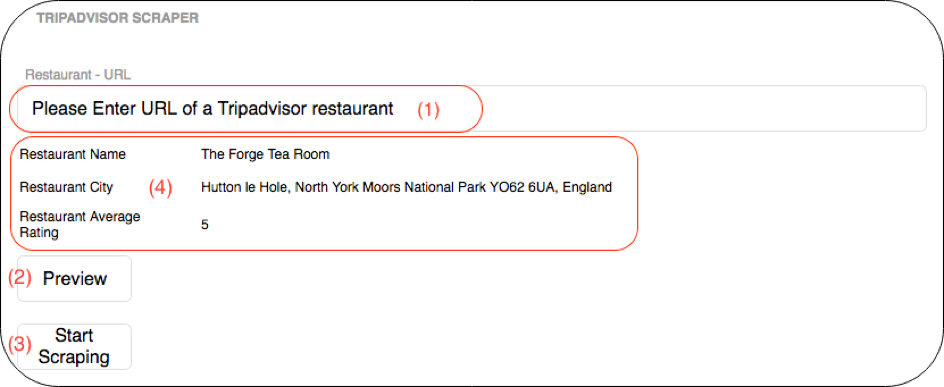
\includegraphics[width=\textwidth]{Bilder/mock-up.png}
					\end{minipage}
					\centering
					\caption[Mock-Up der geplanten Benutzeroberfläche]{Mock-Up der geplanten Benutzeroberfläche}
					\label{pic-mock-up}
				\end{figure}
            
            \begin{itemize}
            \item[(1)] URL-Eingabefeld	\\
            In dieses Feld fügt der Anwender die URL des Restaurants ein, dessen Informationen von Interesse sind.
            \item[(2)] Preview-Button\\
            Durch Klick auf diesen Button wird zunächst geprüft ob im Eingabefeld eine valide Tripadvisor-Restaurant-URL eingegeben wurde. Falls nein, soll eine entsprechende Fehlermeldung dem Nutzer angezeigt werden. Falls ja, soll im mit (4) markierten Bereich die Informationen Restaurantname, Ort und Durchschnittsbewertung angezeigt werden.
            \item[(3)]	Start Scraping-Button\\
            Durch Klick auf diesen Button soll zunächst überprüft werden, ob das betreffende Restaurant bereits in der Datenbank erfasst wurde. Falls ja soll der Vorgang abgebrochen werden und der User erhält eine entsprechende Fehlermeldung. Falls nein wird die Extraktion und anschließende Persistierung in der Datenbank angestoßen. 
            \end{itemize}
			
			\subsection[GUI - Umsetzung - Skanny Morandi]{GUI – Umsetzung}
			In Abbildung \ref{pic-GUI} ist die konkret implementierte GUI des im Rahmen dieser Arbeit erstellten Programms zu sehen. Sie wird bei Ausführung des Programms angezeigt. Das Layout des Mock-Ups konnte weitestgehend umgesetzt werden, das Verhalten wurde wie oben beschrieben umgesetzt. Im Folgenden soll nun die Implementierung der Funktionalitäten näher beschrieben werden.

				\begin{figure}[H]
					\centering
					\begin{minipage}[b]{0.9\textwidth}
						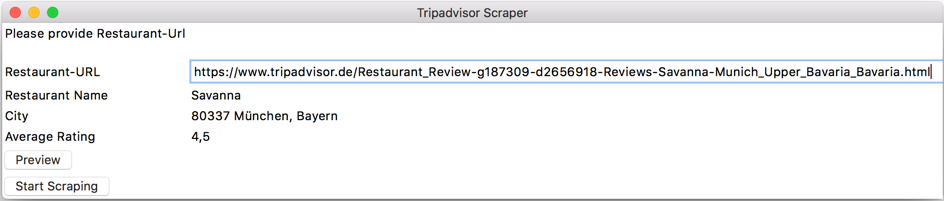
\includegraphics[width=\textwidth]{Bilder/GUI.png}
					\end{minipage}
					\centering
					\caption[Benutzeroberfläche des Tripadvisor Crawlers unter MacOS]{Benutzeroberfläche des Tripadvisor Crawlers unter MacOS}
					\label{pic-GUI}
				\end{figure}

            
            \begin{description}
            \item[Funktionalität - URL-Validierung] Bei betätigen des Preview-Buttons wird der im Textfeld stehende String mit Hilfe der Library ``validators'' über RegEx darauf überprüft, ob er dem Format einer URL im Allgemeinen entspricht. Als nächsten Schritt wird der String darauf geprüft ob er mit\\ ``https://www.tripadvisor.de/Restaurant\_Review'' beginnt. Schlägt eine der beiden Prüfungen fehl wird ein Pop-Up mit entsprechender Fehlermeldung angezeigt. Ist die Prüfung erfolgreich erfolgt werden die Preview-Daten extrahiert
            \item[Funktionalität - Preview] Hier wird ein Teilabschnitt des in Kapitel \ref{implementierung} beschriebenen Scraping Vorgangs über Beautiful-Soup durchgeführt, allerdings wird nicht der gesamte Vorgang durchgeführt sondern es werden aus dem Quellcode der URL lediglich Restaurantname, Ort und Postleitzahl sowie durchschnittliche Bewertungspunktzahl extrahiert und an entsprechender Stelle in der GUI angezeigt.
            \item[Funktionalität – Start Scraping]Es erfolgt eine Prüfung ob es in der Datenbank einen Eintrag mit dem aus der URL-extrahierten Restaurantname und dessen Ort und Postleitzahl gibt. Falls ja wird ein Pop-up angezeigt mit entsprechender Nachricht und der Vorgang wird abgebrochen. Ist es noch nicht vorhanden wird die Extraktion der Restaurant- und Reviewdaten wie in Kapitel \ref{implementierung} angestoßen.




            \end{description}
	
	


	\chapter{Erfüllung der Anforderungen}

		\begin{figure}[H]
					\centering
					\begin{minipage}[b]{0.9\textwidth}
						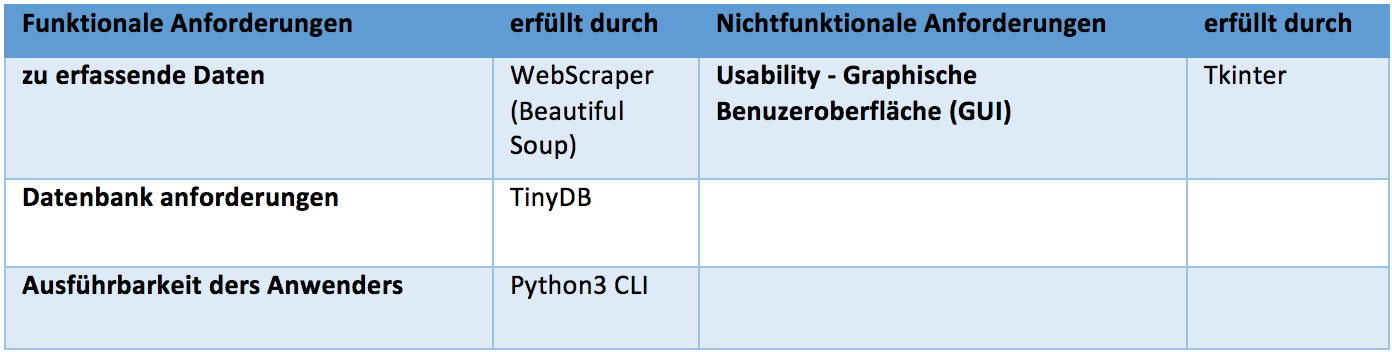
\includegraphics[width=\textwidth]{Bilder/TabErfuellt.png}
					\end{minipage}
					\centering
					\caption[Tabelle der erfüllten Anforderungen]{Tabelle der erfüllten Anforderungen}
					\label{TabErfuellt}
				\end{figure}		
	
		\section[Funktionale Anforderungen - Skanny Morandi]{Funktionale Anforderungen}

		\begin{description}
			\item[Zu erfassende Daten] alle angeforderten Daten der Restaurants sowie deren Bewertungen werden, wie im Detail in Kapitel \ref{implementierung} anschaulich erklärt, mit der Python Library „Beautiful Soup“ erfasst und zur weiteren Verarbeitung verfügbar gemacht

			\item[Datenbank Anforderungen] Wie in Kapitel \ref{datenhaltung} beschrieben, haben sich die Ersteller der Arbeit für den mit Python gut vereinbaren und leichtgewichtigen Datenbank-Typen „TinyDB“ entschieden. Eben da wurde geschildert wie und in welcher Form die extrahierten Daten in einer JSON-Datei presistiert werden und die angestrebten Datenbank-Qualitätsmerkmale bewerkstelligt wurden.

			\item[Ausführbarkeit des Anwenders] Der Anwender des Programms kann, gegeben, dass die Infrastruktur für die Laufbarkeit von Python-Code vorinstalliert ist, das Programm ausführen, über die Kommandozeile eines Terminals in Unix- oder Mac-Systemen oder die Dos-Eingabeaufforderung eines Windowssystems.

			\item[Eingabe einer URL als Input-Parameter] Die Eingabe des Input-Parameters wurde über die in Kapitel \ref{GUI} behandelte GUI und dessen entsprechendes Texteingabefeld bewerkstelligt. So ist es dem User möglich dem Programm den Input-Parameter zu übergeben.

		\end{description}

		\section[Nicht-funktionale Anforderungen - Skanny Morandi]{Nicht-funktionale Anforderungen}
		In Kapitel \ref{GUI} wurde die Implementierung und Konzeption der graphischen Benutzeroberfläche dokumentiert. Über sie ist es möglich die Funktionalitäten des erstellten Programms zu steuern. Der Anwender der Software kann in das dafür vorgesehene Textfeld die URL des zu extrahierenden Restaurants eingeben. Über den Button „Preview“ wird zunächst die Validierung der URL vorgenommen und anschließend werden in der GUI die drei Grundinformationen Name, Ort und Postleitzahl und Durchschnittsbewertung angezeigt. Bei Klick auf „Start Scraping“ wird zunächst geprüft ob das zu extrahierende Restaurant schon in der Datenbank vorhanden ist und beginnt, falls dies nicht der Fall ist, Restaurantdaten und die seiner Reviews zu extrahieren und in der Datenbank zu persistieren.

		
	


	\chapter{Fazit und Ausblick}
	
		\section[Unsere Erfahrungen/Probleme (evtl. API) - Anja Wolf]{Unsere Erfahrungen/Probleme (evtl. API)}

		\section[Wie sind wir damit klargekommen - Anja Wolf]{Wie sind wir damit klargekommen}

	
	
	
	
%						    	Hinzufügen relevanter Verzeichnisse
%   									Abbildungsverzeichnis
	\clearpage
	\addcontentsline{toc}{chapter}{Abbildungsverzeichnis}
	\listoffigures
	
	
	
%   									Programmcodeverzeichnis	
	\clearpage
	%Erneute Bennenung für das Verzeichnis 
	\addcontentsline{toc}{chapter}{Programmcodeverzeichnis}
	\renewcommand{\lstlistingname}{Programmcodeverzeichnis}
	\lstlistoflistings
	\renewcommand{\lstlistlistingname}{\lstlistingname}
	
	
	
%   									Abkürzungsverzeichnis	
%	\chapter*{Abkürzungsverzeichnis}
%		\vspace{1.0cm}
%		\begin{acronym}[SEPSEP]
%			\acro{oem}[OEM]{Original Equipment Manufacturer}
%			\acro{bob}[BOB]{Breakout-Box}
%			\acro{can}[CAN]{Controller Area Network}
%			\acro{lin}[LIN]{Local Interconnect Network}
%			\acro{obd}[OBD]{On-Board-Diagnose}	
%			\acro{sda}[SDA]{Serial Data Line}
%			\acro{scl}[SCL]{Serial Clock Line}
%			\acro{gui}[GUI]{Graphical User Interface}
%			\acro{pdf}[PDF]{Portable Document Format}
			%\acro{SD}[SD]{Secure Digital Memory Card}
			%\acro{pc}[PC]{Personal Computer}
			%\acro{USB}[USB]{Universal Serial Bus}
%		\end{acronym}
%		\addcontentsline{toc}{chapter}{Abkürzungsverzeichnis}
	
	
	
%   									Literaturverzeichnis	
	\clearpage
	\addcontentsline{toc}{chapter}{Literaturverzeichnis}
	\begin{thebibliography}{9} 
		\vspace{1.0cm}
		%Internetrecherche 
		
		\bibitem{bib-atomfeed} Atom Feed\\ Ryte Wiki: Atom Feed, \newline \url{https://de.ryte.com/wiki/Atom_Feed}, aufgerufen am \today
					
		\bibitem{bib-deepweb} Deep Web\\ Advidera: Deep Web, \newline \url{https://www.advidera.com/glossar/deep-web}, aufgerufen am \today	
		
		\bibitem{bib-utf8} Kodierung in UTF-8\\ UTF-8, a transformation format of ISO 10646, \newline \url{https://tools.ietf.org/html/rfc3629}, aufgerufen am \today
		
		\bibitem{bib-tinydb} TinyDB\\ Project Description TinyDB, \newline \url{https://pypi.org/project/tinydb/}, aufgerufen am \today
		
		\bibitem{bib-sqlite} SQLite\\ About SQLite, \newline \url{https://www.sqlite.org/about.html}, aufgerufen am \today
		
		\bibitem{bib-daten} Definition von Datenarten zur konsistenten Kommunikation im Unternehmen\\ Piro A., Gebauer M. Hrsg: \glqq Vieweg und Teubner in Daten- und Informationsqualität.\grqq, S.143 - 156
		
		%7
		\bibitem{bib-webscraping} Practical Web Scraping for Data Science: best practices and examples with Python\\ vanden Broucke S., Baesens B. Hrsg: \O Apress Media LLC: Welmoed Spahr.\grqq
		
		%8
		\bibitem{bib-articlewebscraping} Jan Seipel\\ Webscraping als Methode der Informationsbeschaffung, \newline \url{http://www.vfm-online.de/weblog/wp-content/uploads/2014/01/info7-2016-2\_S15-17.pdf}, aufgerufen am \today
		
		%9
		\bibitem{bib-scrapehero} ScrapeHero\\What is web scraping – Part 1 – Beginner’s guide,\newline \url{https://www.scrapehero.com/a-beginners-guide-to-web-scraping-part-1-the-basics/}, aufgerufen am \today
		
		%10
		\bibitem{bib-anzSterne} Screenshot unbereinigte Daten,\newline \url{https://www.tripadvisor.de/Restaurant\_Review-g187309-d742684-
		Reviews-Hofbraeuhaus-Munich\_Upper\_Bavaria\_Bavaria.html}, aufgerufen am \today
		
		%11
		\bibitem{bib-statista} Umsatz von Tripadvisor weltweit,\newline \url{https://de.statista.com/statistik/daten/studie/543148/umfrage/umsatz-von-tripadvisor-weltweit-nach-quartalen/}, aufgerufen am \today
		
		\bibitem{bib-taMedia} Tripadvisor Mediacenter,\newline \url{https://tripadvisor.mediaroom.com/DE-about-us}, aufgerufen am \today
		
		\bibitem{bib-tripadvisorLogo} Our Logos: TripAdvisor Media Group Logos,\newline \url{https://tripadvisor.mediaroom.com/our-brand}, aufgerufen am \today
		
		\bibitem{bib-taSued} Süddeutsche Zeitung,\newline Bei Kundenbewertungen wird gelogen, was das Zeug hält \newline \url{https://bit.ly/2w1oZqQ}, aufgerufen am \today
		
		\bibitem{bib-webpython} Web scraping with Python: collecting data from the modern web\\ Mitchel, R. Hrsg: \O'Reilly Media, Inc.
		
		\bibitem{bib-bs4} Beautiful Soup Documentation, \newline \url{http://www.crummy.com/software/BeautifulSoup/bs4/doc/} aufgerufen am \today
		
		\bibitem{bib-reviewcontainer} Screenshot Review Container,\newline \url{https://bit.ly/2JC9HAo}, aufgerufen am \today
		
		\bibitem{bib-pipEnv} Python Pipenv \& Virtual Environments,\newline \url{https://bit.ly/2sPKwnw}, aufgerufen am \today
		
		\bibitem{bib-scrapeHero} ScrapeHero,\newline Beginners guide to Web Scraping: Part 2 – Build a web scraper for Reddit using Python and BeautifulSoup \newline \url{https://bit.ly/2JHoVnT}, aufgerufen am \today
		
		\bibitem{bib-tkinterDocu} Tkinter, \newline
		Graphical User Interfaces with Tk\\
		\url{https://docs.python.org/3/library/tk.html}, aufgerufen am aufgerufen am 28.Juni 2018
		
		%Buchrecherche
		%\bibitem{bib-handb} Kraftfahrzeugtechnik \\ Hans-Hermann Braess, Ulrich Seiffert Hrsg: \glqq Vieweg Handbuch Kraftfahrzeugtechnik\grqq, Springer-Vieweg-Verlag, S. 5, 7. Auflage 2013
	\end{thebibliography}
	
	
	
%   									Selbstständigkeitserklärung
	\newpage
	\setstretch{1.5}
	\chapter*{Eidesstattliche Erklärung}
		%\vspace{1.5\textheight}
		Hiermit erklären wir, Johannes Knippel, Anja Wolf, Johanna Sickendiek und Skanny Morandi, dass wir die vorliegende Arbeit mit dem Titel \textit{Extraktion unstrukturierter Daten und Integration in eine Datenbank am Beispiel TripAdvisor} selbstständig verfasst, noch nicht anderweitig für Prüfungszwecke vorgelegt, keine anderen als die angegebenen Quellen oder Hilfsmittel benützt sowie wörtliche und sinngemäße Zitate als solche gekennzeichnet haben.
		\vspace{15mm}
		\\
		\\
		\begin{flushleft}
			\begin{tabular}[H]{ll}
				
				München, den \parbox{5,5cm}{\today}  	& 	\parbox{6cm}{\hrule\medskip \textit{Unterschrift}}\\[2cm]
													  	& 	\parbox{6cm}{\hrule\medskip \textit{Unterschrift}}\\[2cm]
													  	& 	\parbox{6cm}{\hrule\medskip \textit{Unterschrift}}\\[2cm]
													  	& 	\parbox{6cm}{\hrule\medskip \textit{Unterschrift}}\\[2cm]
			\end{tabular}
		\end{flushleft}
		\addcontentsline{toc}{chapter}{Eidesstattliche Erklärung}


\end{document}
%The End
%Johannes Knippel